\documentclass[11pt,oneside]{article}
\pdfminorversion=7
\usepackage{QuizStyle}
\hypersetup{
    pdftitle={20260922 Quiz for MATH230 Probability \& Statistics},
    pdfauthor={Jungwoo Kim},
    pdfsubject={Quiz for MATH230 Probability \& Statistics},
    pdfcreator={LaTeX}
}
\begin{document}
\quiztitle{20260922 Quiz}
\begin{exercise}{3.1}
Classify each random variable as discrete or continuous: $X$, the annual number of car accidents in Virginia; $Y$, the duration of 18 holes of golf; $M$, annual milk yield of one cow; $N$, eggs laid by a hen in a month; $P$, monthly building permits issued in a city; $Q$, weight of grain harvested per acre.
\end{exercise}

\begin{solution}
The counts $X,N,P$ are \boxed{\text{discrete}}. The measurements $Y,M,Q$ are \boxed{\text{continuous}} (in the usual measurement models).
\end{solution}

\begin{exercise}{3.3}
A coin is tossed three times. Let $W$ be the number of heads minus the number of tails. List the sample space and assign a value of $W$ to every outcome.
\end{exercise}

\begin{solution}
\[
\begin{array}{c@{\qquad}cccccccc}\toprule
\omega&HHH&HHT&HTH&THH&HTT&THT&TTH&TTT\\\midrule
W(\omega)&3&1&1&1&-1&-1&-1&-3\\\bottomrule
\end{array}
\]
The eight outcomes displayed in the table constitute the sample space $S$.
\end{solution}

\begin{exercise}{3.4}
A fair coin is tossed until two consecutive heads appear. List every possible terminal outcome requiring at most six tosses. Is the complete sample space discrete? Explain.
\end{exercise}

\begin{solution}
The terminal strings of length at most six are
\[
\begin{gathered}
HH,\ THH,\ HTHH,\ TTHH,\ HTTHH,\ THTHH,\ TTTHH,\\
HTHTHH,\ HTTTHH,\ THTTHH,\ TTHTHH,\ TTTTHH.
\end{gathered}
\]
Each string ends in $HH$ with no earlier consecutive $HH$. The complete sample space is countably infinite and is therefore \boxed{\text{discrete}}.
\end{solution}

\Needspace{10\baselineskip}
\begin{exercise}{3.5}
Find the normalization constant $c$ for each discrete pmf on $x=0,1,2$:
\par
\begin{exercisesubparts}
\item $p_X(x)=c(x^2+4)$;
\item $\displaystyle p_X(x)=c\binom{3}{x}\binom{3}{3-x}$. 
\end{exercisesubparts}
\end{exercise}

\begin{solution}
\begin{align*}
\textup{(a)}\quad&1=c(4+5+8),&c&=\boxed{\frac1{17}},\\
\textup{(b)}\quad&1=c(1+9+9),&c&=\boxed{\frac1{19}}.
\end{align*}
\end{solution}

\begin{exercise}{3.8}
A coin is tossed three times independently, with a head twice as likely as a tail. Let $W$ be the number of heads minus the number of tails. Find the probability distribution of $W$.
\end{exercise}

\begin{solution}
Here $\Prob(H)=2/3$ and $\Prob(T)=1/3$. The number of heads is binomial with parameters $3$ and $2/3$, and $W=2H-3$. Thus
\[
\begin{array}{c|rrrr}\toprule
w&-3&-1&1&3\\\midrule
p_W(w)&1/27&6/27&12/27&8/27\\\bottomrule
\end{array}
\]
\end{solution}

\begin{exercise}{3.9}
A continuous response proportion $X$ has density $f_X(x)=2(x+2)/5$ for $0<x<1$, and zero otherwise.
\begin{exercisesubparts}
\item Verify that it is a density.
\item Find $\Prob(1/4<X<3/4)$.
\end{exercisesubparts}
\end{exercise}

\begin{solution}
\begin{align*}
\textup{(a)}\quad&\int_0^1\frac{2(x+2)}5\,\dd x
=\frac25\left[\frac{x^2}{2}+2x\right]_0^1=\boxed{1},\\
\textup{(b)}\quad&\int_{1/4}^{3/4}\frac{2(x+2)}5\,\dd x
=\boxed{\frac12}.
\end{align*}
\end{solution}

\begin{exercise}{3.11}
Of seven television sets, two are defective. A hotel chooses three sets uniformly without replacement. Find the probability distribution of $X$, the number of defective sets purchased, and display its probability histogram.
\end{exercise}

\begin{solution}
The hypergeometric counting formula gives
\[
p_X(x)=\frac{\binom{2}{x}\binom{5}{3-x}}{\binom{7}{3}},\quad x=0,1,2.
\]
Hence $p_X(0)=2/7$, $p_X(1)=4/7$, and $p_X(2)=1/7$. The corresponding probability histogram is
\begin{center}
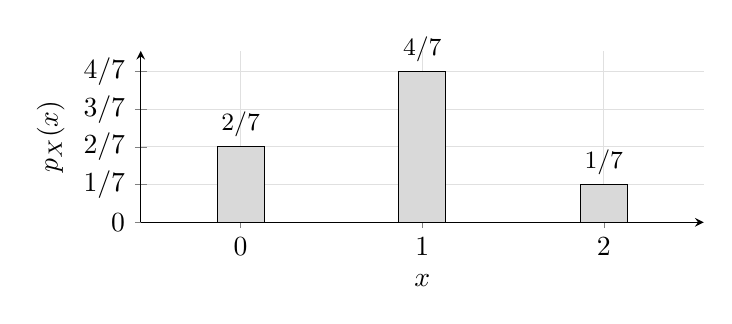
\begin{tikzpicture}
\begin{axis}[
 width=0.72\textwidth,height=0.31\textwidth,
 ybar,bar width=17pt,xmin=-0.55,xmax=2.55,ymin=0,ymax=0.65,
 xtick={0,1,2},ytick={0,0.142857,0.285714,0.428571,0.571429},
 yticklabels={$0$,$1/7$,$2/7$,$3/7$,$4/7$},
 xlabel={$x$},ylabel={$p_X(x)$},
 axis lines=left,grid=major,grid style={black!12},
 nodes near coords,point meta=explicit symbolic,
 every node near coord/.append style={font=\small,anchor=south}]
\addplot[fill=gray!30,draw=black] table[meta=label,row sep=\\]{x y label\\ 0 0.285714 $2/7$\\ 1 0.571429 $4/7$\\ 2 0.142857 $1/7$\\};
\end{axis}
\end{tikzpicture}
\end{center}
\end{solution}

\begin{exercise}{3.12}
The maturity $T$ (years) of a bond has cumulative distribution function
\[
F_T(t)=\begin{cases}
0,&t<1,\\1/4,&1\le t<3,\\1/2,&3\le t<5,\\3/4,&5\le t<7,\\1,&t\ge7.
\end{cases}
\]
Find:
\begin{exercisesubparts}
\item $\Prob(T=5)$.
\item $\Prob(T>3)$.
\item $\Prob(1.4<T<6)$.
\item $\Prob(T\le5\mid T\ge2)$.
\end{exercisesubparts}
\end{exercise}

\begin{solution}
The jumps at $t=1,3,5,7$ are each $1/4$. Therefore
\begin{align*}
\textup{(a)}\quad&\boxed{1/4},&
\textup{(b)}\quad&\boxed{1/2},\\
\textup{(c)}\quad&\boxed{1/2},&
\textup{(d)}\quad&\frac{\Prob(T=3\text{ or }5)}{\Prob(T=3,5,\text{ or }7)}=\boxed{2/3}.
\end{align*}
\end{solution}

\begin{exercise}{3.13}
The number $X$ of imperfections per 10 meters of synthetic fabric has pmf
\[
\begin{array}{c|rrrrr}\toprule
x&0&1&2&3&4\\\midrule
p_X(x)&0.41&0.37&0.16&0.05&0.01\\\bottomrule
\end{array}
\]
Construct its cdf.
\end{exercise}

\begin{solution}
Summing the probabilities up to each point gives
\[
F_X(x)=\begin{cases}
0,&x<0,\\0.41,&0\le x<1,\\0.78,&1\le x<2,\\0.94,&2\le x<3,\\0.99,&3\le x<4,\\1,&x\ge4.
\end{cases}
\]
\end{solution}

\begin{exercise}{3.14}
The waiting time $X$ (hours) between speeders has cdf $F_X(x)=0$ for $x<0$ and $F_X(x)=1-e^{-4x}$ for $x\ge0$. Find the probability of a wait of less than 12 minutes:
\begin{exercisesubparts}
\item from the cdf.
\item from the pdf.
\end{exercisesubparts}
\end{exercise}

\begin{solution}
Since 12 minutes is $1/5$ hour,
\begin{align*}
\textup{(a)}\quad&F_X(1/5)=\boxed{1-e^{-4/5}},\\
\textup{(b)}\quad&\int_0^{1/5}4e^{-4x}\,\dd x=\boxed{1-e^{-4/5}}.
\end{align*}
Both values are about $0.5507$.
\end{solution}

\begin{exercise}{3.17}
The continuous variable $X$ has constant density $f_X(x)=1/2$ for $1<x<3$, and zero otherwise.
\begin{exercisesubparts}
\item Verify normalization.
\item Find $\Prob(2<X<2.5)$.
\item Find $\Prob(X\le1.6)$.
\end{exercisesubparts}
\end{exercise}

\begin{solution}
\begin{align*}
\textup{(a)}\quad&\int_1^3\frac12\,\dd x=\boxed{1},\\
\textup{(b)}\quad&\int_2^{5/2}\frac12\,\dd x=\boxed{\frac14},\\
\textup{(c)}\quad&\int_1^{8/5}\frac12\,\dd x=\boxed{\frac3{10}}.
\end{align*}
\end{solution}

\begin{exercise}{3.18}
The density of $X$ is $f_X(x)=2(1+x)/27$ for $2<x<5$, and zero otherwise. Find:
\begin{exercisesubparts}
\item $\Prob(X<4)$.
\item $\Prob(3\le X<4)$.
\end{exercisesubparts}
\end{exercise}

\begin{solution}
An antiderivative is $(x^2+2x)/27$. Thus
\begin{align*}
\textup{(a)}\quad&\left[\frac{x^2+2x}{27}\right]_2^4=\boxed{\frac{16}{27}},\\
\textup{(b)}\quad&\left[\frac{x^2+2x}{27}\right]_3^4=\boxed{\frac13}.
\end{align*}
\end{solution}

\begin{exercise}{3.21}
Let $f_X(x)=k\sqrt{x}$ for $0\le x<4$, and zero otherwise.
\begin{exercisesubparts}
\item Determine $k$.
\item Obtain $F_X(x)$ and calculate $\Prob(3<X<4)$.
\end{exercisesubparts}
\end{exercise}

\begin{solution}
\noindent\textup{(a)} Normalization gives
\[
1=k\int_0^4\sqrt{x}\,\dd x=\frac{16}{3}k,
\]
so $\boxed{k=3/16}$.\par\medskip
\noindent\textup{(b)} The cdf is
\[
F_X(x)=\begin{cases}
0,&x<0,\\x^{3/2}/8,&0\le x<4,\\1,&x\ge4.
\end{cases}
\]
Therefore $\Prob(3<X<4)=1-F_X(3)=\boxed{1-3\sqrt3/8}$.
\end{solution}

\begin{exercise}{3.23}
A biased coin has $\Prob(H)=2/3$ and is tossed three times independently. Let $W$ be heads minus tails. Determine its cdf and use it to calculate:
\begin{exercisesubparts}
\item $\Prob(W>0)$.
\item $\Prob(-1\le W<3)$.
\end{exercisesubparts}
\end{exercise}

\begin{solution}
As $W$ takes $-3,-1,1,3$ with respective probabilities $1/27,6/27,12/27,8/27$,
\[
F_W(w)=\begin{cases}
0,&w<-3,\\1/27,&-3\le w<-1,\\7/27,&-1\le w<1,\\19/27,&1\le w<3,\\1,&w\ge3.
\end{cases}
\]
Hence
\[
\textup{(a)}\quad\boxed{\Prob(W>0)=\frac{20}{27}},\qquad
\textup{(b)}\quad\boxed{\Prob(-1\le W<3)=\frac23}.
\]
\end{solution}

\begin{exercise}{3.27}
An electronic component has lifetime density $f_X(x)=e^{-x/1000}/1000$ for $x\ge0$, and zero otherwise.
\begin{exercisesubparts}
\item Find $F_X(x)$.
\item Find the probability of surviving beyond 1000 hours.
\item Find the probability of failing before 2000 hours.
\end{exercisesubparts}
\end{exercise}

\begin{solution}
\noindent\textup{(a)} For $x\ge0$,
\[
F_X(x)=\int_0^x\frac{e^{-t/1000}}{1000}\,\dd t=1-e^{-x/1000},
\]
and $F_X(x)=0$ for $x<0$.\par\medskip
\noindent\textup{(b)} The probability of surviving beyond 1000 hours is $\boxed{e^{-1}}$.\par\medskip
\noindent\textup{(c)} The probability of failing before 2000 hours is $\boxed{1-e^{-2}}$.
\end{solution}

\begin{exercise}{3.28}
The weight $X$ (ounces) of cereal in a box has density $f_X(x)=2/5$ for $23.75\le x\le26.25$, and zero otherwise.
\begin{exercisesubparts}
\item Verify the density.
\item Find $\Prob(X<24)$.
\item Find $\Prob(X>26)$.
\end{exercisesubparts}
\end{exercise}

\begin{solution}
\begin{align*}
\textup{(a)}\quad&\frac25(26.25-23.75)=\boxed{1},\\
\textup{(b)}\quad&\frac25(24-23.75)=\boxed{0.10},\\
\textup{(c)}\quad&\frac25(26.25-26)=\boxed{0.10}.
\end{align*}
\end{solution}

\begin{exercise}{3.30}
Measurements of physical systems are subject to variation, and modeling measurement error is important in statistics. Suppose that the error $X$ in measuring a physical quantity has density $f_X(x)=k(3-x^2)$ on $-1\le x\le1$, and zero otherwise.
\begin{exercisesubparts}
\item Determine $k$.
\item Calculate $\Prob(X<1/2)$.
\item Calculate $\Prob(|X|>0.8)$.
\end{exercisesubparts}
\end{exercise}

\begin{solution}
\[
1=k\int_{-1}^1(3-x^2)\,\dd x=\frac{16k}{3},\qquad \boxed{k=\frac3{16}}.
\]
Consequently,
\begin{align*}
\textup{(b)}\quad&\frac3{16}\int_{-1}^{1/2}(3-x^2)\,\dd x=\boxed{\frac{99}{128}},\\
\textup{(c)}\quad&2\cdot\frac3{16}\int_{4/5}^{1}(3-x^2)\,\dd x=\boxed{\frac{41}{250}}.
\end{align*}
\end{solution}

\begin{exercise}{3.32}
A company's proportion $Y$ of its budget devoted to pollution control has density $f_Y(y)=5(1-y)^4$ on $0\le y\le1$, and zero elsewhere. Verify that this is a density and find $\Prob(Y<0.10)$ and $\Prob(Y>0.50)$.
\end{exercise}

\begin{solution}
\begin{align*}
\textup{(a)}\quad&\int_0^1 5(1-y)^4\,\dd y=\boxed{1},\\
\textup{(b)}\quad&1-(0.90)^5=\boxed{0.40951},\\
\textup{(c)}\quad&(0.50)^5=\boxed{\frac1{32}}.
\end{align*}
\end{solution}

\begin{exercise}{3.36}
The variable $X$ has density $f_X(x)=2(1-x)$ on $0<x<1$, and zero elsewhere. Find:
\begin{exercisesubparts}
\item $\Prob(X<0.5)$.
\item $\Prob(X>0.4)$.
\item $\Prob(X<0.7\mid X\ge0.5)$.
\end{exercisesubparts}
\end{exercise}

\begin{solution}
Since $\Prob(X\ge t)=(1-t)^2$ for $0\le t\le1$,
\begin{align*}
\textup{(a)}\quad&1-(0.5)^2=\boxed{0.75},\\
\textup{(b)}\quad&(0.6)^2=\boxed{0.36},\\
\textup{(c)}\quad&\frac{(0.5)^2-(0.3)^2}{(0.5)^2}=\boxed{0.64}.
\end{align*}
\end{solution}

\begin{exercise}{3.37}
Find the constants $c$ for which the following joint mass functions are normalized:
\par
\begin{exercisesubparts}
\item $p_{X,Y}(x,y)=cxy$, for $x,y\in\{1,2\}$;
\item $p_{X,Y}(x,y)=c|x-y|$, for $x\in\{-2,0,2\}$, $y\in\{-3,3\}$. 
\end{exercisesubparts}
\end{exercise}

\begin{solution}
\begin{align*}
\textup{(a)}\quad&1=c\left(\sum_{x=1}^2x\right)^2=9c,
&\boxed{c=1/9},\\
\textup{(b)}\quad&1=c(1+5+3+3+5+1)=18c,
&\boxed{c=1/18}.
\end{align*}
\end{solution}

\begin{exercise}{3.38}
The joint mass function is $p_{X,Y}(x,y)=(x+y)/30$ for $x=0,1,2,3$ and $y=0,1,2$ (zero elsewhere). Find
\par
\begin{exercisesubparts}
\item $\Prob(X\le1,Y=1)$;
\item $\Prob(X>1,Y\le1)$;
\item $\Prob(X\le Y)$;
\item $\Prob(X+Y=2)$.
\end{exercisesubparts}
\end{exercise}

\begin{solution}
Summing the indicated joint masses,
\begin{align*}
\textup{(a)}\quad&\frac{(0+1)+(1+1)}{30}=\boxed{\frac1{10}},\\
\textup{(b)}\quad&\frac{(2+0)+(2+1)+(3+0)+(3+1)}{30}=\boxed{\frac25},\\
\textup{(c)}\quad&\frac{(0+1)+(1+1)+(0+2)+(1+2)+(2+2)}{30}=\boxed{\frac25},\\
\textup{(d)}\quad&\frac{(0+2)+(1+1)+(2+0)}{30}=\boxed{\frac15}.
\end{align*}
\end{solution}

\begin{exercise}{3.39}
A random sample of four fruits is drawn without replacement from three oranges, two apples, and three bananas. Let $X$ and $Y$ be the numbers of oranges and apples selected.
Find:
\begin{exercisesubparts}
\item the joint pmf explicitly.
\item $\Prob(X+Y\le2)$.
\end{exercisesubparts}
\end{exercise}

\begin{solution}
\textup{(a)} The joint mass is
\[
\boxed{p_{X,Y}(x,y)=\frac{\binom{3}{x}\binom{2}{y}\binom{3}{4-x-y}}{\binom{8}{4}}}
\]
for integers $0\le x\le3$, $0\le y\le2$, $1\le x+y\le4$, and $p_{X,Y}(x,y)=0$ otherwise.
\noindent\textup{(b)} The event $X+Y\le2$ means at least two bananas are drawn, so
\[
\Prob(X+Y\le2)
=\frac{\binom{3}{2}\binom{5}{2}+\binom{3}{3}\binom{5}{1}}{\binom{8}{4}}
=\frac{35}{70}=\boxed{\frac12}.
\]
\end{solution}

\begin{exercise}{3.40}
The proportions of time a fast-food restaurant's drive-through and walk-in services are busy are $X$ and $Y$. Their joint density is $f_{X,Y}(x,y)=\frac23(x+2y)$ on $0<x<1$, $0<y<1$, and zero otherwise. Find:
\begin{exercisesubparts}
\item $f_X$.
\item $f_Y$.
\item $\Prob(X<1/2)$.
\end{exercisesubparts}
\end{exercise}

\begin{solution}
\noindent\textup{(a)} Integrating over $y$ gives
\[
\boxed{f_X(x)=\frac23(x+1)},\qquad 0<x<1.
\]
\noindent\textup{(b)} Integrating over $x$ gives
\[
\boxed{f_Y(y)=\frac13(1+4y)},\qquad 0<y<1.
\]
Both densities are zero outside $(0,1)$.\par\medskip
\noindent\textup{(c)} Therefore
\[
\Prob(X<1/2)=\int_0^{1/2}\frac23(x+1)\,\dd x=\boxed{\frac5{12}}.
\]
\end{solution}

\begin{exercise}{3.41}
In a one-kilogram box of chocolates, $X$ and $Y$ are the weights in kilograms of creams and toffees; the remainder is cordials. Assume the joint density $f_{X,Y}(x,y)=24xy$ for $x,y\ge0$, $x+y\le1$, and zero elsewhere. Find
\par
\begin{exercisesubparts}
\item the probability that cordials exceed half the box weight;
\item the marginal density of $X$;
\item $\Prob(Y<1/8\mid X=3/4)$.
\end{exercisesubparts}
\end{exercise}

\begin{solution}
\textup{(a)} Cordials exceed $1/2$ precisely when $X+Y<1/2$. Since the integrand is homogeneous of degree two, scaling the triangle by $1/2$ multiplies the integral by $(1/2)^4$; hence $\boxed{1/16}$.\par\medskip
\noindent\textup{(b)}
\[
f_X(x)=\int_0^{1-x}24xy\,\dd y=\boxed{12x(1-x)^2},\quad 0<x<1.
\]
\noindent\textup{(c)} With $X=3/4$, the conditional support of $Y$ is $(0,1/4)$ and its conditional density is proportional to $y$. Therefore
\[
\Prob(Y<1/8\mid X=3/4)=\frac{(1/8)^2}{(1/4)^2}=\boxed{\frac14}.
\]
\end{solution}

\begin{exercise}{3.42}
The lifetimes $X$ and $Y$ (years) of two components have joint density $f_{X,Y}(x,y)=e^{-(x+y)}$ for $x,y>0$, and zero otherwise. Find $\Prob(1<X<2\mid Y=2)$.
\end{exercise}

\begin{solution}
The joint density factorizes into two exponential marginals, so $X$ and $Y$ are independent. Therefore
\[
\Prob(1<X<2\mid Y=2)=\int_1^2e^{-x}\,\dd x=\boxed{e^{-1}-e^{-2}}.
\]
\end{solution}

\begin{exercise}{3.43}
Let $X$ be a reaction time (seconds) and $Y$ a temperature. Their joint density is $f_{X,Y}(x,y)=4xy$ on $0<x<1$, $0<y<1$ and zero elsewhere. Find:
\begin{exercisesubparts}
\item $\Prob(0\le X\le1/2,\ 1/4\le Y\le1/2)$.
\item $\Prob(X<Y)$.
\end{exercisesubparts}
\end{exercise}

\begin{solution}
The density factorizes as $(2x)(2y)$, and the marginals have the same form. Thus
\begin{align*}
\textup{(a)}\quad&\left(\int_0^{1/2}2x\,\dd x\right)
\left(\int_{1/4}^{1/2}2y\,\dd y\right)
=\boxed{\frac3{64}},\\
\textup{(b)}\quad&\int_0^1\int_0^y4xy\,\dd x\,\dd y
=\boxed{\frac12}.
\end{align*}
\end{solution}

\begin{exercise}{3.46}
The joint pmf $p_{X,Y}(x,y)=(x+y)/30$ is supported on $x\in\{0,1,2,3\}$ and $y\in\{0,1,2\}$. Find the marginal pmfs of $X$ and $Y$.
\end{exercise}

\begin{solution}
\begin{align*}
p_X(x)&=\sum_{y=0}^2\frac{x+y}{30}=\boxed{\frac{x+1}{10}},\quad x=0,1,2,3,\\
p_Y(y)&=\sum_{x=0}^3\frac{x+y}{30}=\boxed{\frac{3+2y}{15}},\quad y=0,1,2.
\end{align*}
Both functions are zero outside their displayed supports.
\end{solution}

\begin{exercise}{3.47}
For the daily amount $Y$ of kerosene available and the amount $X$ sold (both in thousands of liters), the joint density is $f_{X,Y}(x,y)=2$ for $0<x\le y<1$, and zero otherwise.
\begin{exercisesubparts}
\item Are $X,Y$ independent?
\item Find $\Prob(1/4<X<1/2\mid Y=3/4)$.
\end{exercisesubparts}
\end{exercise}

\begin{solution}
\textup{(a)} The triangular support rules out independence. Indeed, $f_X(x)=2(1-x)$ and $f_Y(y)=2y$, while $f_{X,Y}(x,y)$ is not their product. Thus $\boxed{\text{dependent}}$.\par\medskip
\noindent\textup{(b)} Since $f_{X\mid Y}(x\mid y)=1/y$ for $0<x<y$,
\[
\Prob(1/4<X<1/2\mid Y=3/4)=\int_{1/4}^{1/2}\frac4{3}\,\dd x=\boxed{\frac13}.
\]
\end{solution}

\begin{exercise}{3.48}
A random sample of four fruits is drawn without replacement from three oranges, two apples, and three bananas. Let $X$ and $Y$ be the numbers of oranges and apples selected. The joint pmf is
\[
p_{X,Y}(x,y)=\frac{\binom{3}{x}\binom{2}{y}\binom{3}{4-x-y}}{\binom{8}{4}}
\]
for admissible integer pairs $(x,y)$, and zero otherwise.
Find:
\begin{exercisesubparts}
\item the conditional pmf $p_{Y\mid X}(y\mid2)$.
\item $\Prob(Y=0\mid X=2)$.
\end{exercisesubparts}
\end{exercise}

\begin{solution}
\noindent\textup{(a)} For $X=2$, the unnormalized counts for $Y=0,1,2$ are $9,18,3$, totaling $30$. Thus
\[
\boxed{p_{Y\mid X}(y\mid2)=\begin{cases}3/10,&y=0,\\3/5,&y=1,\\1/10,&y=2,\\0,&\text{otherwise},\end{cases}}
\]
\par\medskip
\noindent\textup{(b)} Hence $\boxed{\Prob(Y=0\mid X=2)=3/10}$.
\end{solution}

\begin{exercise}{3.49}
The joint pmf of the number $X$ of machine malfunctions and the number $Y$ of technician calls is
\[
\begin{array}{c@{\qquad}ccc}\toprule
p_{X,Y}(x,y)&x=1&x=2&x=3\\\midrule
y=1&0.05&0.05&0.10\\
y=3&0.05&0.10&0.35\\
y=5&0.00&0.20&0.10\\\bottomrule
\end{array}
\]
Find:
\begin{exercisesubparts}
\item the marginal pmf of $X$.
\item that of $Y$.
\item $\Prob(Y=3\mid X=2)$.
\end{exercisesubparts}
\end{exercise}

\begin{solution}
\noindent\textup{(a)} Summing over $y$ gives the marginal of $X$:
\[
\begin{array}{c@{\qquad}ccc}\toprule
x&1&2&3\\\midrule p_X(x)&0.10&0.35&0.55\\\bottomrule
\end{array}
\]
\noindent\textup{(b)} Summing over $x$ gives the marginal of $Y$:
\[
\begin{array}{c@{\qquad}ccc}\toprule
y&1&3&5\\\midrule p_Y(y)&0.20&0.50&0.30\\\bottomrule
\end{array}
\]
\noindent\textup{(c)} Therefore $\Prob(Y=3\mid X=2)=0.10/0.35=\boxed{2/7}$.
\end{solution}

\begin{exercise}{3.50}
The joint pmf of $X,Y$ is
\[
\begin{array}{c@{\qquad}cc}\toprule
p_{X,Y}(x,y)&x=2&x=4\\\midrule
y=1&0.10&0.15\\
y=3&0.20&0.30\\
y=5&0.10&0.15\\\bottomrule
\end{array}
\]
Find the marginal pmfs of $X$ and $Y$.
\end{exercise}

\begin{solution}
The marginal distributions are
\[
\begin{aligned}
&p_X(2)=0.40,\qquad p_X(4)=0.60,\\
&p_Y(1)=0.25,\quad p_Y(3)=0.50,\quad p_Y(5)=0.25.
\end{aligned}
\]
Both pmfs are zero elsewhere.
\end{solution}

\begin{exercise}{3.52}
A coin is tossed twice independently with $\Prob(H)=0.30$. Let $Z$ be the indicator of heads on the first toss, and $W$ the total number of heads. Find:
\begin{exercisesubparts}
\item the joint pmf of $(W,Z)$.
\item the marginal pmf of $W$.
\item the marginal pmf of $Z$.
\item the probability of at least one head.
\end{exercisesubparts}
\end{exercise}

\begin{solution}
\noindent\textup{(a)} The outcomes $HH,HT,TH,TT$ have probabilities $0.09,0.21,0.21,0.49$, respectively. Therefore
\[
\begin{array}{c@{\qquad}cc}\toprule
p_{W,Z}(w,z)&z=0&z=1\\\midrule
w=0&0.49&0\\
w=1&0.21&0.21\\
w=2&0&0.09\\\bottomrule
\end{array}
\]
\noindent\textup{(b)} The marginal pmf of $W$ is $p_W(0)=0.49$, $p_W(1)=0.42$, $p_W(2)=0.09$.\par\medskip
\noindent\textup{(c)} The marginal pmf of $Z$ is $p_Z(0)=0.70$, $p_Z(1)=0.30$.\par\medskip
\noindent\textup{(d)} Finally,
\[
\Prob(W\ge1)=1-\Prob(W=0)=\boxed{0.51}.
\]
\end{solution}

\begin{exercise}{3.53}
The joint density of $X$ and $Y$ is $f_{X,Y}(x,y)=(6-x-y)/8$ for $0<x<2$ and $2<y<4$, and zero otherwise. Find $\Prob(1<Y<3\mid X=1.5)$.
\end{exercise}

\begin{solution}
Since
\[
f_X(x)=\int_2^4\frac{6-x-y}{8}\,\dd y=\frac{3-x}{4},
\]
the conditional density at $x=3/2$ is
\[
f_{Y\mid X}(y\mid3/2)=\frac{(9/2-y)/8}{(3-3/2)/4}=\frac{9/2-y}{3},\quad2<y<4.
\]
Thus
\[
\Prob(1<Y<3\mid X=3/2)=\int_2^3\frac{9/2-y}{3}\,\dd y=\boxed{\frac23}.
\]
\end{solution}

\begin{exercise}{3.54}
For the joint pmf
\[
\begin{array}{c@{\qquad}ccc}\toprule
p_{X,Y}(x,y)&x=1&x=2&x=3\\\midrule
y=1&0.05&0.05&0.10\\
y=3&0.05&0.10&0.35\\
y=5&0.00&0.20&0.10\\\bottomrule
\end{array}
\]
Determine whether $X$ and $Y$ are independent.
\end{exercise}

\begin{solution}
The marginals satisfy $p_X(1)=0.10$ and $p_Y(1)=0.20$, but
\[
p_{X,Y}(1,1)=0.05\ne(0.10)(0.20)=0.02.
\]
Therefore $\boxed{X\text{ and }Y\text{ are dependent}}$.
\end{solution}

\begin{exercise}{3.55}
For the joint pmf
\[
\begin{array}{c@{\qquad}cc}\toprule
p_{X,Y}(x,y)&x=2&x=4\\\midrule
y=1&0.10&0.15\\
y=3&0.20&0.30\\
y=5&0.10&0.15\\\bottomrule
\end{array}
\]
Determine whether $X$ and $Y$ are independent.
\end{exercise}

\begin{solution}
The marginal probabilities are
\[
p_X(2)=0.40,\quad p_X(4)=0.60,
\qquad (p_Y(1),p_Y(3),p_Y(5))=(0.25,0.50,0.25).
\]
Every joint mass equals the product of the corresponding marginals. Hence
\[\boxed{X\text{ and }Y\text{ are independent}.}\]
\end{solution}

\begin{exercise}{3.56}
The joint density of $X,Y$ is $f_{X,Y}(x,y)=6x$ for $0<x<1$, $0<y<1-x$, and zero otherwise.
\begin{exercisesubparts}
\item Show dependence.
\item Find $\Prob(X>0.3\mid Y=0.5)$.
\end{exercisesubparts}
\end{exercise}

\begin{solution}
\textup{(a)} The joint density has triangular support, unlike the product of two positive marginals on a rectangle. Therefore the variables are \boxed{\text{dependent}}.\par\medskip
\noindent\textup{(b)} The conditional density for $Y=1/2$ is proportional to $x$ on $0<x<1/2$. Thus
\[
\Prob(X>0.3\mid Y=0.5)
=\frac{\int_{0.3}^{0.5}x\,\dd x}{\int_0^{0.5}x\,\dd x}
=\boxed{0.64}.
\]
\end{solution}

\begin{exercise}{3.57}
The joint density is $f_{X,Y,Z}(x,y,z)=kxy^2z$ on $0<x<1$, $0<y<1$, $0<z<2$, and zero otherwise.
\begin{exercisesubparts}
\item Determine $k$.
\item Find $\Prob(X<1/4,Y>1/2,1<Z<2)$.
\end{exercisesubparts}
\end{exercise}

\begin{solution}
\noindent\textup{(a)} Normalization gives
\[
1=k\left(\frac12\right)\left(\frac13\right)(2)=\frac k3,
\quad\boxed{k=3}.
\]
\noindent\textup{(b)} The density factors, so
\[
\Prob(X<1/4,Y>1/2,1<Z<2)
=\left(\frac1{16}\right)\left(\frac78\right)\left(\frac34\right)
=\boxed{\frac{21}{512}}.
\]
\end{solution}

\begin{exercise}{3.60}
The joint density of $X,Y,Z$ is $f_{X,Y,Z}(x,y,z)=\frac49xyz^2$ for $0<x,y<1$ and $0<z<3$, and zero otherwise. Find
\par
\begin{exercisesubparts}
\item the joint marginal density of $(X,Y)$;
\item the marginal density of $Z$;
\item $\Prob(1/4<X<1/2, Y>1/3, 2<Z<3)$;
\item $\Prob(0<Z<2\mid X=1/2,Y=1/2)$. 
\end{exercisesubparts}
\end{exercise}

\begin{solution}
\begin{align*}
\textup{(a)}\quad&f_{X,Y}(x,y)=\int_0^3\frac49xyz^2\,\dd z=\boxed{4xy},\\
\textup{(b)}\quad&f_Z(z)=\int_0^1\int_0^1\frac49xyz^2\,\dd x\,\dd y=\boxed{\frac{z^2}{9}}.
\end{align*}
These apply on $0<x,y<1$ and $0<z<3$ respectively, and vanish elsewhere. The density factors, giving
\begin{align*}
\textup{(c)}\quad&\left(\frac3{16}\right)\left(\frac89\right)\left(\frac{19}{27}\right)=\boxed{\frac{19}{162}},\\
\textup{(d)}\quad&\int_0^2\frac{z^2}{9}\,\dd z=\boxed{\frac8{27}}.
\end{align*}
\end{solution}

\begin{exercise}{3.61}
A one-unit tobacco blend contains Turkish and domestic tobacco in proportions $X,Y$, with the remainder being other tobacco. Their joint density is $f_{X,Y}(x,y)=24xy$ for $x,y\ge0$, $x+y\le1$, and zero elsewhere. Find:
\begin{exercisesubparts}
\item $\Prob(X>1/2)$.
\item the marginal density of $Y$.
\item $\Prob(X<1/8\mid Y=3/4)$.
\end{exercisesubparts}
\end{exercise}

\begin{solution}
\textup{(a)} The marginal is $f_X(x)=12x(1-x)^2$, so
\[
\Prob(X>1/2)=\int_{1/2}^1 12x(1-x)^2\,\dd x=\boxed{\frac5{16}}.
\]
\noindent\textup{(b)} Integrating over $0<x<1-y$,
\[
f_Y(y)=\int_0^{1-y}24xy\,\dd x=\boxed{12y(1-y)^2},\quad0<y<1.
\]
\noindent\textup{(c)} With $Y=3/4$, the conditional density of $X$ is proportional to $x$ on $(0,1/4)$, so
\[
\Prob(X<1/8\mid Y=3/4)=\left(\frac{1/8}{1/4}\right)^2=\boxed{\frac14}.
\]
\end{solution}

\begin{exercise}{3.68}
The joint density is $f_{X,Y}(x,y)=(3x-y)/11$ on $1<x<3$ and $0<y<1$, and zero elsewhere.
\begin{exercisesubparts}
\item Find the marginal densities.
\item Check independence.
\item Find $\Prob(X>2)$.
\end{exercisesubparts}
\end{exercise}

\begin{solution}
\textup{(a)} Integrating gives
\[
f_X(x)=\boxed{\frac{3x-1/2}{11}},\quad1<x<3;
\qquad f_Y(y)=\boxed{\frac{12-2y}{11}},\quad0<y<1.
\]
Both vanish outside their stated supports.\par\medskip
\noindent\textup{(b)} The density $(3x-y)/11$ does not factor into these marginals, so $\boxed{\text{dependent}}$.\par\medskip
\noindent\textup{(c)}
\[
\Prob(X>2)=\int_2^3\frac{3x-1/2}{11}\,\dd x=\boxed{\frac7{11}}.
\]
\end{solution}

\Needspace{15\baselineskip}
\begin{exercise}{3.75}
A chemical blend has component proportions $X_1$ and $X_2$ with joint density $f(x_1,x_2)=2$ for $0<x_1<x_2<1$, and zero otherwise.
\begin{exercisesubparts}
\item Find $f_{X_1}$.
\item Find $f_{X_2}$.
\item Calculate $\Prob(X_1<0.2,X_2>0.5)$.
\item Determine $f_{X_1\mid X_2}(x_1\mid x_2)$.
\end{exercisesubparts}
\end{exercise}

\begin{solution}
\begin{align*}
\textup{(a)}\quad&f_{X_1}(x_1)=\int_{x_1}^1 2\,\dd x_2=\boxed{2(1-x_1)},\quad0<x_1<1,\\
\textup{(b)}\quad&f_{X_2}(x_2)=\int_0^{x_2}2\,\dd x_1=\boxed{2x_2},\quad0<x_2<1,\\
\textup{(c)}\quad&\int_{1/2}^1\int_0^{1/5}2\,\dd x_1\,\dd x_2=\boxed{\frac15},\\
\textup{(d)}\quad&f_{X_1\mid X_2}(x_1\mid x_2)=\frac2{2x_2}=\boxed{\frac1{x_2}},\quad0<x_1<x_2<1.
\end{align*}
\end{solution}

\end{document}
